\documentclass[../../main.tex]{subfiles}

\graphicspath{{../../image/}{../../figure/}}

\begin{document}

\subsection{表示学习与潜空间插值}\label{subsection:ch17-表示学习}

我们已经看到，GAN 能胜任生成式模型的工作，它也可用于\textbf{表示学习}（representation learning）（参见\cref{subsection:ch06-表示学习}），其通过无监督学习揭示了数据集中丰富的统计结构。当用\cref{figure:ch17-DCGAN}所示的深度卷积 GAN 在一个卧室图像数据集上进行训练，并且从潜空间中随机抽取样本，然后通过已训练的网络加以传播时，生成的图像看起来也像卧室，正如我们预期的那样（Radford, Metz and Chintala, 2015）。此外，潜空间已经以具有语义意义的方式组织起来。例如，如果我们沿着潜空间中的平滑轨迹进行跟踪，并生成相应的一系列图像，就可以实现从一个图像到另一个图像的平滑过渡，如\cref{figure:ch17-潜空间插值}所示。

\begin{figure}[htbp]
  \centering
  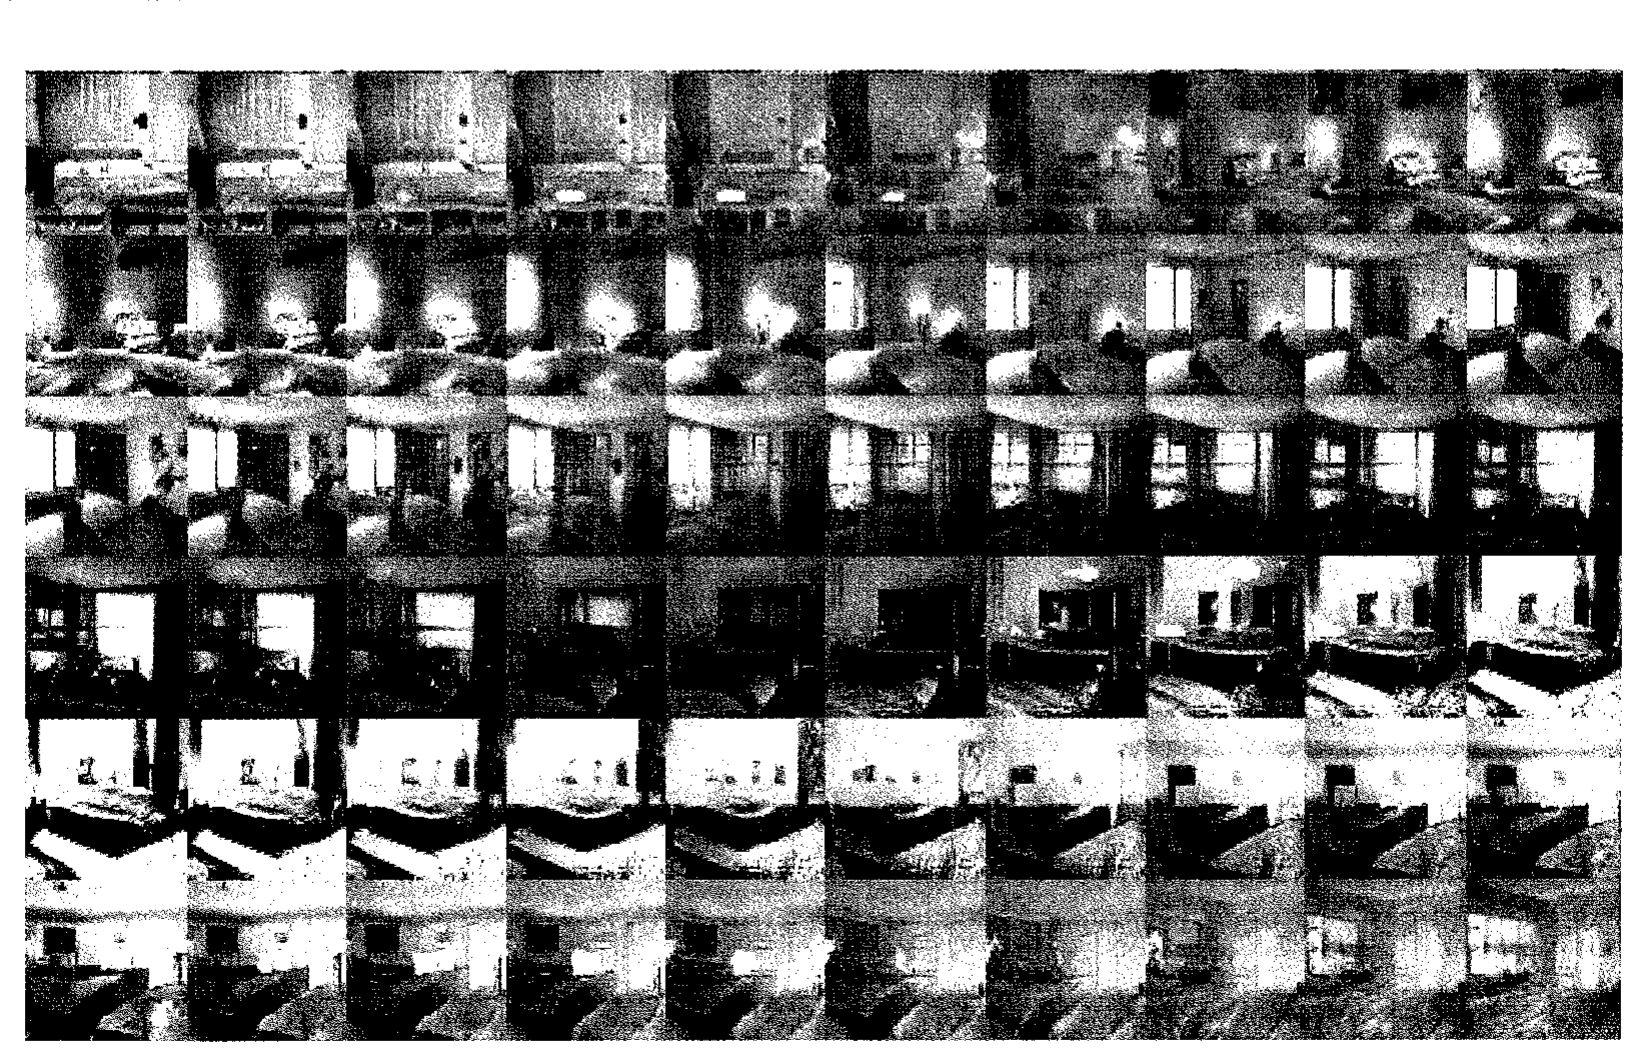
\includegraphics[width=0.95\textwidth]{ch17-fig491-latent-sweep.png}
  \caption{由在卧室图像上训练的深度卷积 GAN 生成的样本。其中的每一行都是通过在潜空间内部随机生成的位置之间进行平滑移动得到的。图像的过渡很平滑，每幅图像看起来都像是一个合理的卧室。在最下方一行，我们看到墙上的电视逐渐变形成了窗户［Radford, Metz, and Chintala (2015)，经授权使用］}
  \label{figure:ch17-潜空间插值}
\end{figure}

此外，识别潜空间中与具有语义意义的变换相对应的方向也是可能的。例如，对人脸图像，某个方向可能对应面部朝向的变化，而其他方向可能对应光照变化或面部微笑程度的变化，这称为\textbf{解耦表示}（disentangled representation）。我们可以利用它们来合成具有特定属性的新图像。

\begin{definition}[解耦表示]\label{definition:ch17-解耦表示}
设 $z\mapsto g(z)$ 是训练好的生成器。若潜空间中存在若干方向 $v_1,\cdots,v_m$，使得沿每个 $v_i$ 移动时，生成的图像中只有第 $i$ 个语义属性（如面部朝向、光照、是否微笑）发生系统性变化，而其余属性近似保持不变，则称该潜空间给出了这些属性的\textbf{解耦表示}（disentangled representation），并称 $v_i$ 为该属性对应的\textbf{语义方向}。
\end{definition}

% SUPPLEMENT: parent=definition:ch17-解耦表示; kind=motivation; location=紧随其后的 remark（重构新增）
\begin{remark}（重构新增）
解耦表示的用途是“可控生成”：找到语义方向之后，就可以固定其余坐标、只沿该方向移动，从而在保持其他属性不变的前提下改变目标属性。这在数据空间中往往做不到——像素级的向量加减会破坏图像的对齐与光照，\cref{figure:ch17-向量算术}最下一行正是这种失败的例子；而潜空间中的移动天然保持“像一张人脸”，因为整个潜空间都被生成器映到数据流形附近。

条件方面要强调：解耦不是 GAN 训练目标的推论，而是额外的结构假设。\cref{proposition:ch17-最优判别器}只保证 $p_g=p_{\mathrm{data}}$，它并不惩罚潜坐标与语义属性之间的纠缠。若训练数据中“戴眼镜”与“男性”高度相关，那么这两个因素在潜空间中对应的方向几乎重合，任何沿其中一个方向的移动都会同时改变两者；只有数据中的相关性足够弱、或额外加入独立性正则时，才可能得到近似解耦的表示。此外，语义方向没有唯一性：不同的随机初始化会给出不同的基，它们能解释同一组属性，因此“找到方向”总是指相对于某个已训练模型而言。
\end{remark}

\begin{example}[ 人脸潜空间中的向量算术]\label{example:ch17-向量算术}
\cref{figure:ch17-向量算术}是一个关于在面部图像上训练的 GAN 的例子，可以看到性别或“戴眼镜与否”等语义属性对应于潜空间中特定的方向。
\end{example}

\begin{figure}[htbp]
  \centering
  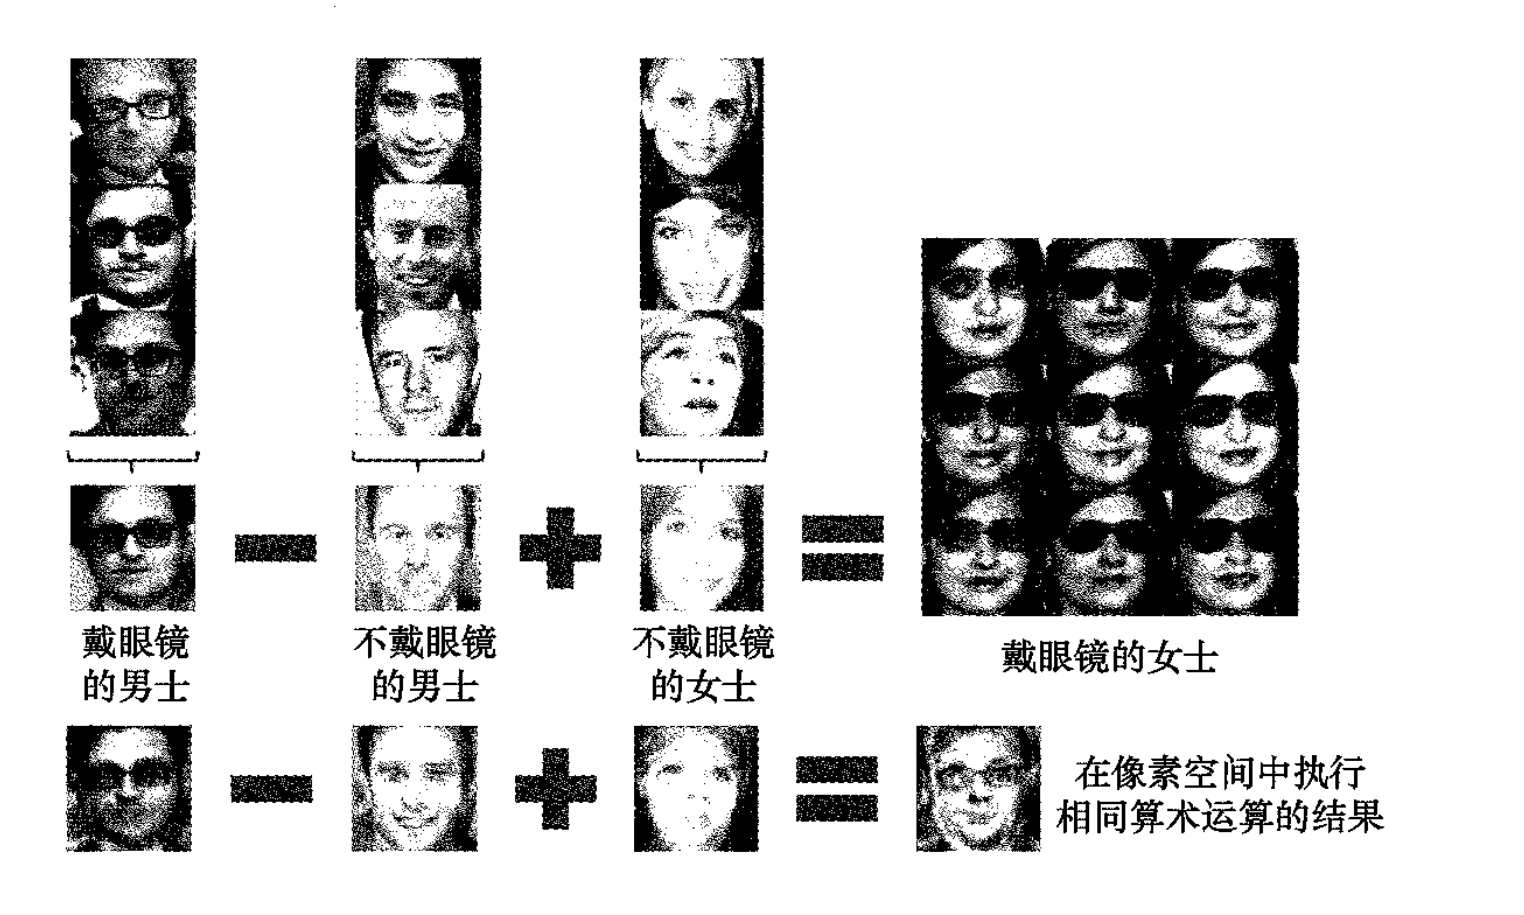
\includegraphics[width=0.8\textwidth]{ch17-fig492-vec-arith.png}
  \caption{在训练成功的 GAN 的潜空间中进行向量运算的例子。对左侧三列中的每一列，算法先对生成这些图像的潜空间向量取平均值，再对具有中间值的结果进行向量运算，这样就创建了右侧 $3\times3$ 阵列中正中的那个新向量。然后向这个向量中添加噪声，产生周围的 $8$ 个样本图像。最下方一行的 $4$ 幅图像则展示了直接在数据空间中应用相同的运算会导致不对齐，从而产生模糊的图像［Radford, Metz, and Chintala (2015)，经授权使用］}
  \label{figure:ch17-向量算术}
\end{figure}

\end{document}
